\section{Metodi con intelligenza artificiale}

    \begin{frame}{Autoencoder}
        \begin{figure}[t!]
            \centering
            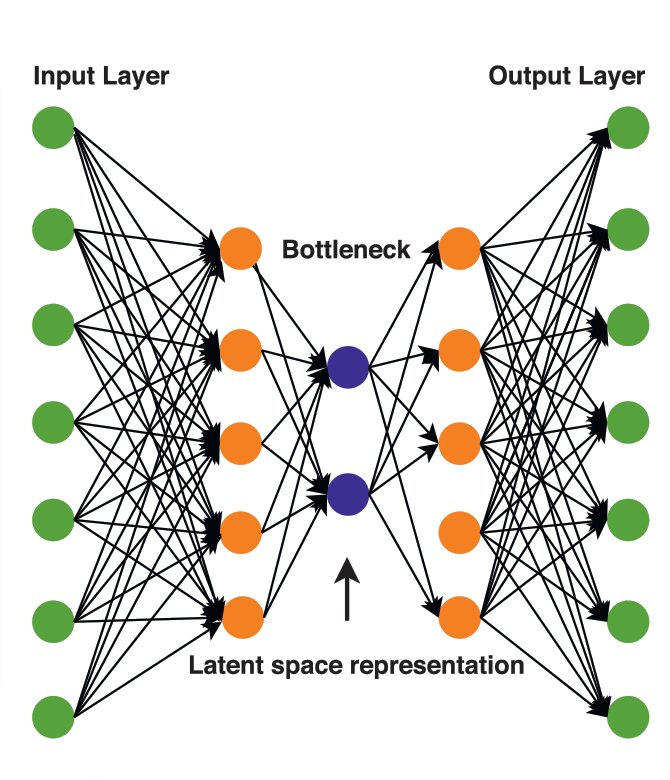
\includegraphics[width=0.5\textheight]{Immagini/Autoencoder_scheme.png}
            \caption{Schema generico di un autoencoder, immagine presa dal documento \cite{mishra2022deep}}
            \label{fig:schemeAutoencoder}
        \end{figure}
    \end{frame}

    \begin{frame}{Metodi con intelligenza artificiale}
        I metodi di codifica con intelligenza artificiale analizzati in questo studio sono i seguenti
        \begin{itemize}
            \item Ballé et al. \cite{minnen2018joint}
            \item Cheng et al. \cite{cheng2020learned}
            \item Wang et al. \cite{wang2022neural} 
        \end{itemize}
    \end{frame}

    \begin{frame}{Ballé et al. 2018}
        \begin{figure}[!h]
            \centering
            \includegraphics[width=0.7\textheight]{Immagini/Ballé2018_Rete.png}
            \caption{Diagramma rete Ballè 2018 et al., immagine presa dal documento \cite{minnen2018joint}}
            \label{fig:balle2018Network}
        \end{figure}
    \end{frame}

    \begin{frame}{Cheng et al. 2020}
        \begin{figure}[!h]
            \centering
            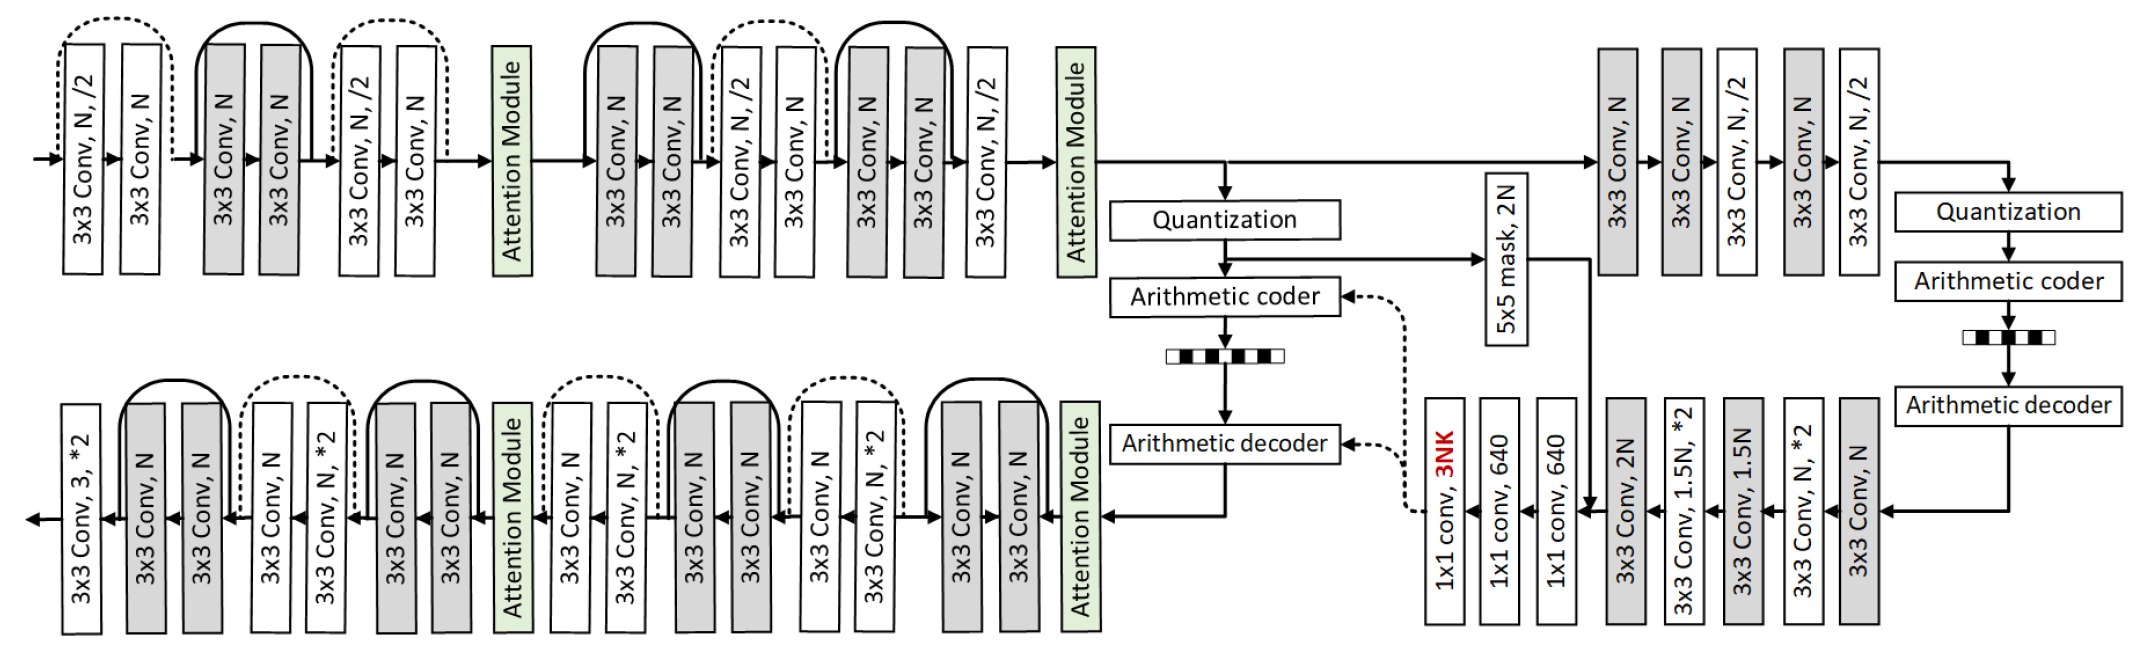
\includegraphics[width=1\textwidth]{Immagini/Cheng2020_Rete.png}
            \caption{Diagramma rete Cheng 2020 et al., immagine presa dal documento \cite{cheng2020learned}}
            \label{fig:cheng2020Network}
        \end{figure}
    \end{frame}

    \begin{frame}{Wang et al. 2022}
        \begin{figure}[!h]
            \centering
            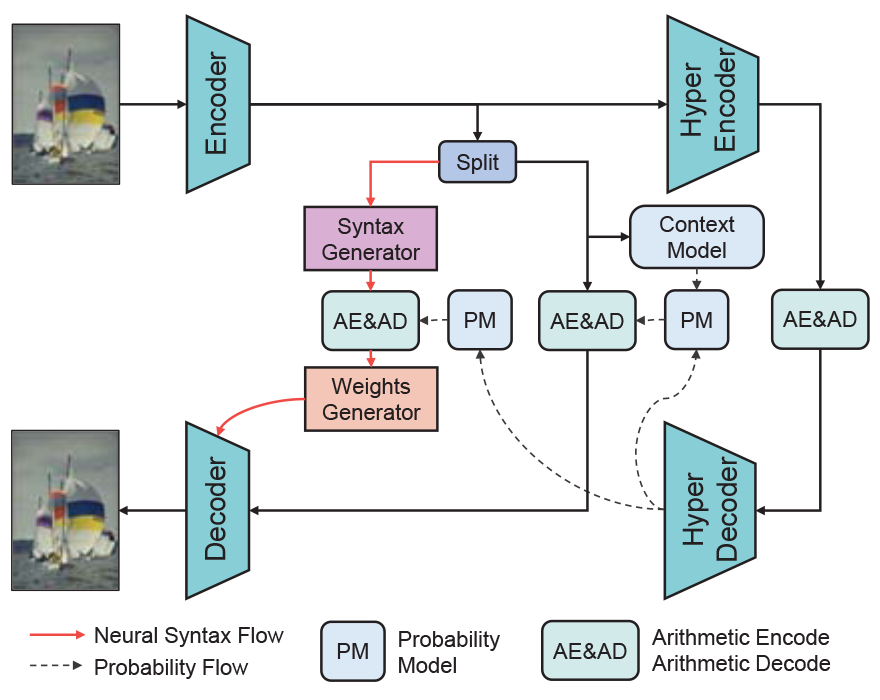
\includegraphics[width=0.6\textheight]{Immagini/Wang2022_Rete.png}
            \caption{Diagramma rete Wang 2022 et al., immagine presa dal documento \cite{wang2022neural}}
            \label{fig:Wang2022Network}
        \end{figure}
    \end{frame}
    